\documentclass{article}
\usepackage[margin=1in]{geometry}
\usepackage{hyperref}
\usepackage{graphicx}
\usepackage{multicol}
\setlength{\parindent}{0in}
\setlength{\parskip}{1em}
\begin{document}

\centerline{\bf CSCI 321, 3D Game Specs, Spring 2015}

{\bf Due date: Wednesday, May 20, Midnight}

Reread the pygame specifications for general things I'll look for in
a game.  However, since 3D is generally {\em much} harder than 2D,
much less is expected of your game.  

If you've used images, sounds, or other resources, make sure you pack
them into your blend file with the
\verb+File->External Data->Pack into .blend file+ menu item.

Set up a new screen layout, called {\bf PlayGame}, by pressing the
\fbox{+}-key on the drop-down menu that has the builtin screen layouts
(Default, Animation, {\em etc.}), renaming it, and then setting it up
with just one large 3D window on the left, and a narrow text window on
the right, as in this figure:

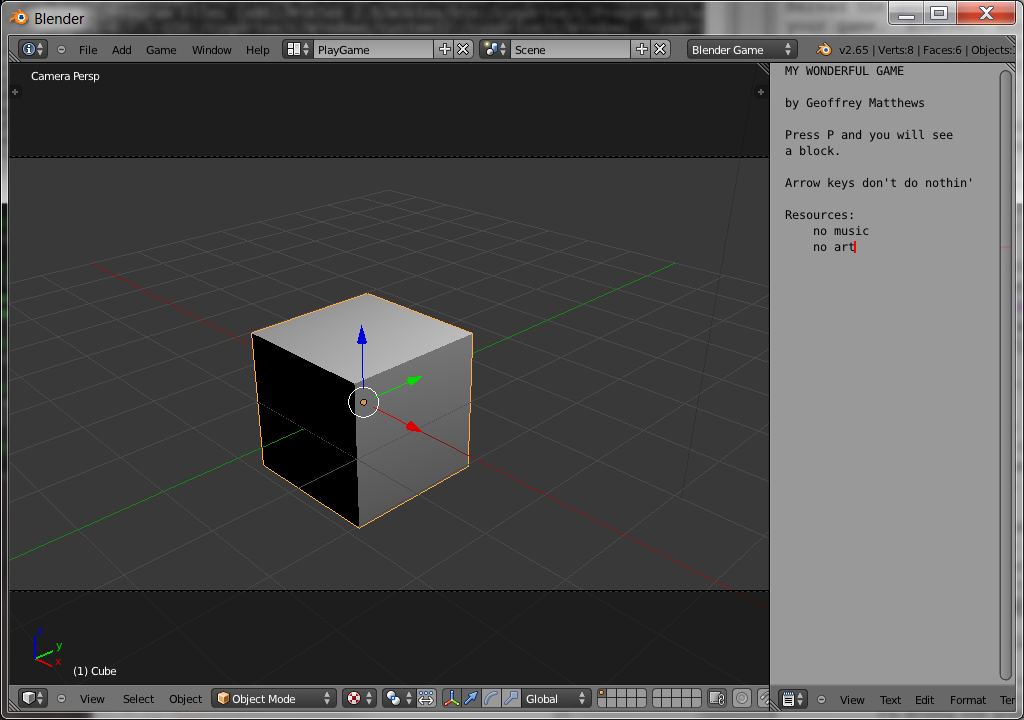
\includegraphics[width=\textwidth]{screenlayout.png}

Set up the 3D window so it is ready to play with a single press of the
P-key: material mode, camera view, {\em etc.}  You can provide your
name, the name of the game, in-game help, and other documentation in
the text window, so that the manual does not have to be consulted.

Also produce a user's manual, as before, nicely formatted.
Please let me know here all the special features
and glorious whatnots you put in your game; tell me what you spent
your time on, so I won't miss it when I'm deciding your grade.
A programmer's guide is not necessary unless you wrote a lot of code
for your game. 

\end{document}
\end
